%% ****** Start of file aiptemplate.tex ****** %
%%
%%   This file is part of the files in the distribution of AIP substyles for REVTeX4.
%%   Version 4.1 of 9 October 2009.
%%
%
% This is a template for producing documents for use with 
% the REVTEX 4.1 document class and the AIP substyles.
% 
% Copy this file to another name and then work on that file.
% That way, you always have this original template file to use.

\documentclass[aip,rsi]{revtex4-1}
\usepackage{graphicx}
%\documentclass[aip,reprint]{revtex4-1}

%\draft % marks overfull lines with a black rule on the right

\begin{document}

% Use the \preprint command to place your local institutional report number 
% on the title page in preprint mode.
% Multiple \preprint commands are allowed.
%\preprint{}

\title{High Resolution Time of Flight Mass Spectrometer for Measuring Products in Heterogenous Catalysis in Higly Sensitive Microreactors} %Title of paper

% repeat the \author .. \affiliation  etc. as needed
% \email, \thanks, \homepage, \altaffiliation all apply to the current author.
% Explanatory text should go in the []'s, 
% actual e-mail address or url should go in the {}'s for \email and \homepage.
% Please use the appropriate macro for the type of information

% \affiliation command applies to all authors since the last \affiliation command. 
% The \affiliation command should follow the other information.

\author{T. Andersen}
\author{R. Jensen}
\author{....}
\affiliation{CINF, Department of Physics...}
\author{O. Hansen}
\affiliation{CINF, Department of Micro- and Nanotechnology}
\author{I. Chorkendorff}
\email[]{ibchork@fysik.dtu.dk}
\affiliation{CINF, Department of Physics...}
%\homepage[]{Your web page}
%\thanks{}
%\altaffiliation{}
%\affiliation{}

% Collaboration name, if desired (requires use of superscriptaddress option in \documentclass). 
% \noaffiliation is required (may also be used with the \author command).
%\collaboration{}
%\noaffiliation

\date{\today}

\begin{abstract}
We demonstrate a combined microreactor and time of flight system for testing and characterization of heterogeneous catalyst with high resolution mass spectrometry and high sensitivity. Catalyst testing is performed in microreactors which have high sensitivity and fast thermal response. Gas analysis is performed with a time of flight mass spectrometer with a modified nude Bayard-Alpert ionization gauge as gas ionization source with a mass resolution of $\Delta$m/m$>$2500. The system design is superior to conventional batch and flow reactors not only due to the high sensitivity, fast temperature response and high mass resolution but also allows to measure on wide mass ranges (0--5000\,amu in the current configuration). As demonstration of the system we here present data from ammonia oxidation on platinum thin films showing resolved spectra of OH$^{-}$ and NH$_{3}^{+}$.
\end{abstract}

\pacs{}% insert suggested PACS numbers in braces on next line

\maketitle %\maketitle must follow title, authors, abstract and \pacs

% Body of paper goes here. Use proper sectioning commands. 
% References should be done using the \cite, \ref, and \label commands
\section{Introduction}
In heterogeneous catalysis the optimization and development of equipment is important both to minimize the cost of equipment but also to be able to study complicated systems. As a platform for testing heterogeneous catalysts microfabricated reactors or microreactors have been found suitable due to both high surface-to-volume ratio, fast temperature response and minimization of thermal and concentration gradients. Such a platform have been developed in our department \cite{Henriksen2009}. However, a suitable reactor platform is only part of the task; reactant and product detection and characterization is essential to determine catalyst performance. Typically, quadrupole mass spectrometers (QMSs) are used in low pressure regimes to analyze gas composition while gas chromatographs are used for high pressure measurements. The QMS, however, suffer from a low mass resolution ($\Delta$m/m$\sim$200) which makes analysis of complicated spectra difficult and cumbersome. The QMS is additionally subject to a low mass range (typically up to $\sim$500\,amu) limiting general use. Furthermore, QMSs are typically operated by logging a single (or a few) masses as a function of time to increase the time resolution. This in turn limits the ability to acquire full mass spectra continuously during the experiment. Gas chromatographs have inherently low time resolution which make them unsuitable for fast time response measurements as in the case of microreactors and is in general difficult to use as mass spectrometers. As an alternative to the gas chromatography or QMSs, time of flight mass spectrometers (TOF-MS) offer both high mass resolution ($\Delta$m/m$>$400) and fast acquisition of full mass spectra ($>$1\,Hz) along with mass range only limited by the detector. For a typical microchannel plate (MCP) a mass range of (0--5000\,amu) can be obtained. Until now, to our knowledge, the testing of catalysts in a microreactor with subsequent gas analysis by a TOF-MS have not been demonstrated. Here we describe a microreactor and TOF-MS system which combines the high sensitivity of microreactors and the high mass resolution TOF-MSs for testing and characterizing heterogeneous catalysts.

\section{System design}
The microreactor as a reactor and TOF as a mass spectrometer enables high sensitivity reactivity measurements of the catalyst under investigation combined with high resolution mass spectrometry. The catalyst under investigation is deposited in the microreactor from where reaction products are detected with time of flight mass spectrometry. A schematic of the entire setup is shown in Figure \ref{fig:TOF_microreactor}.
\begin{figure}
 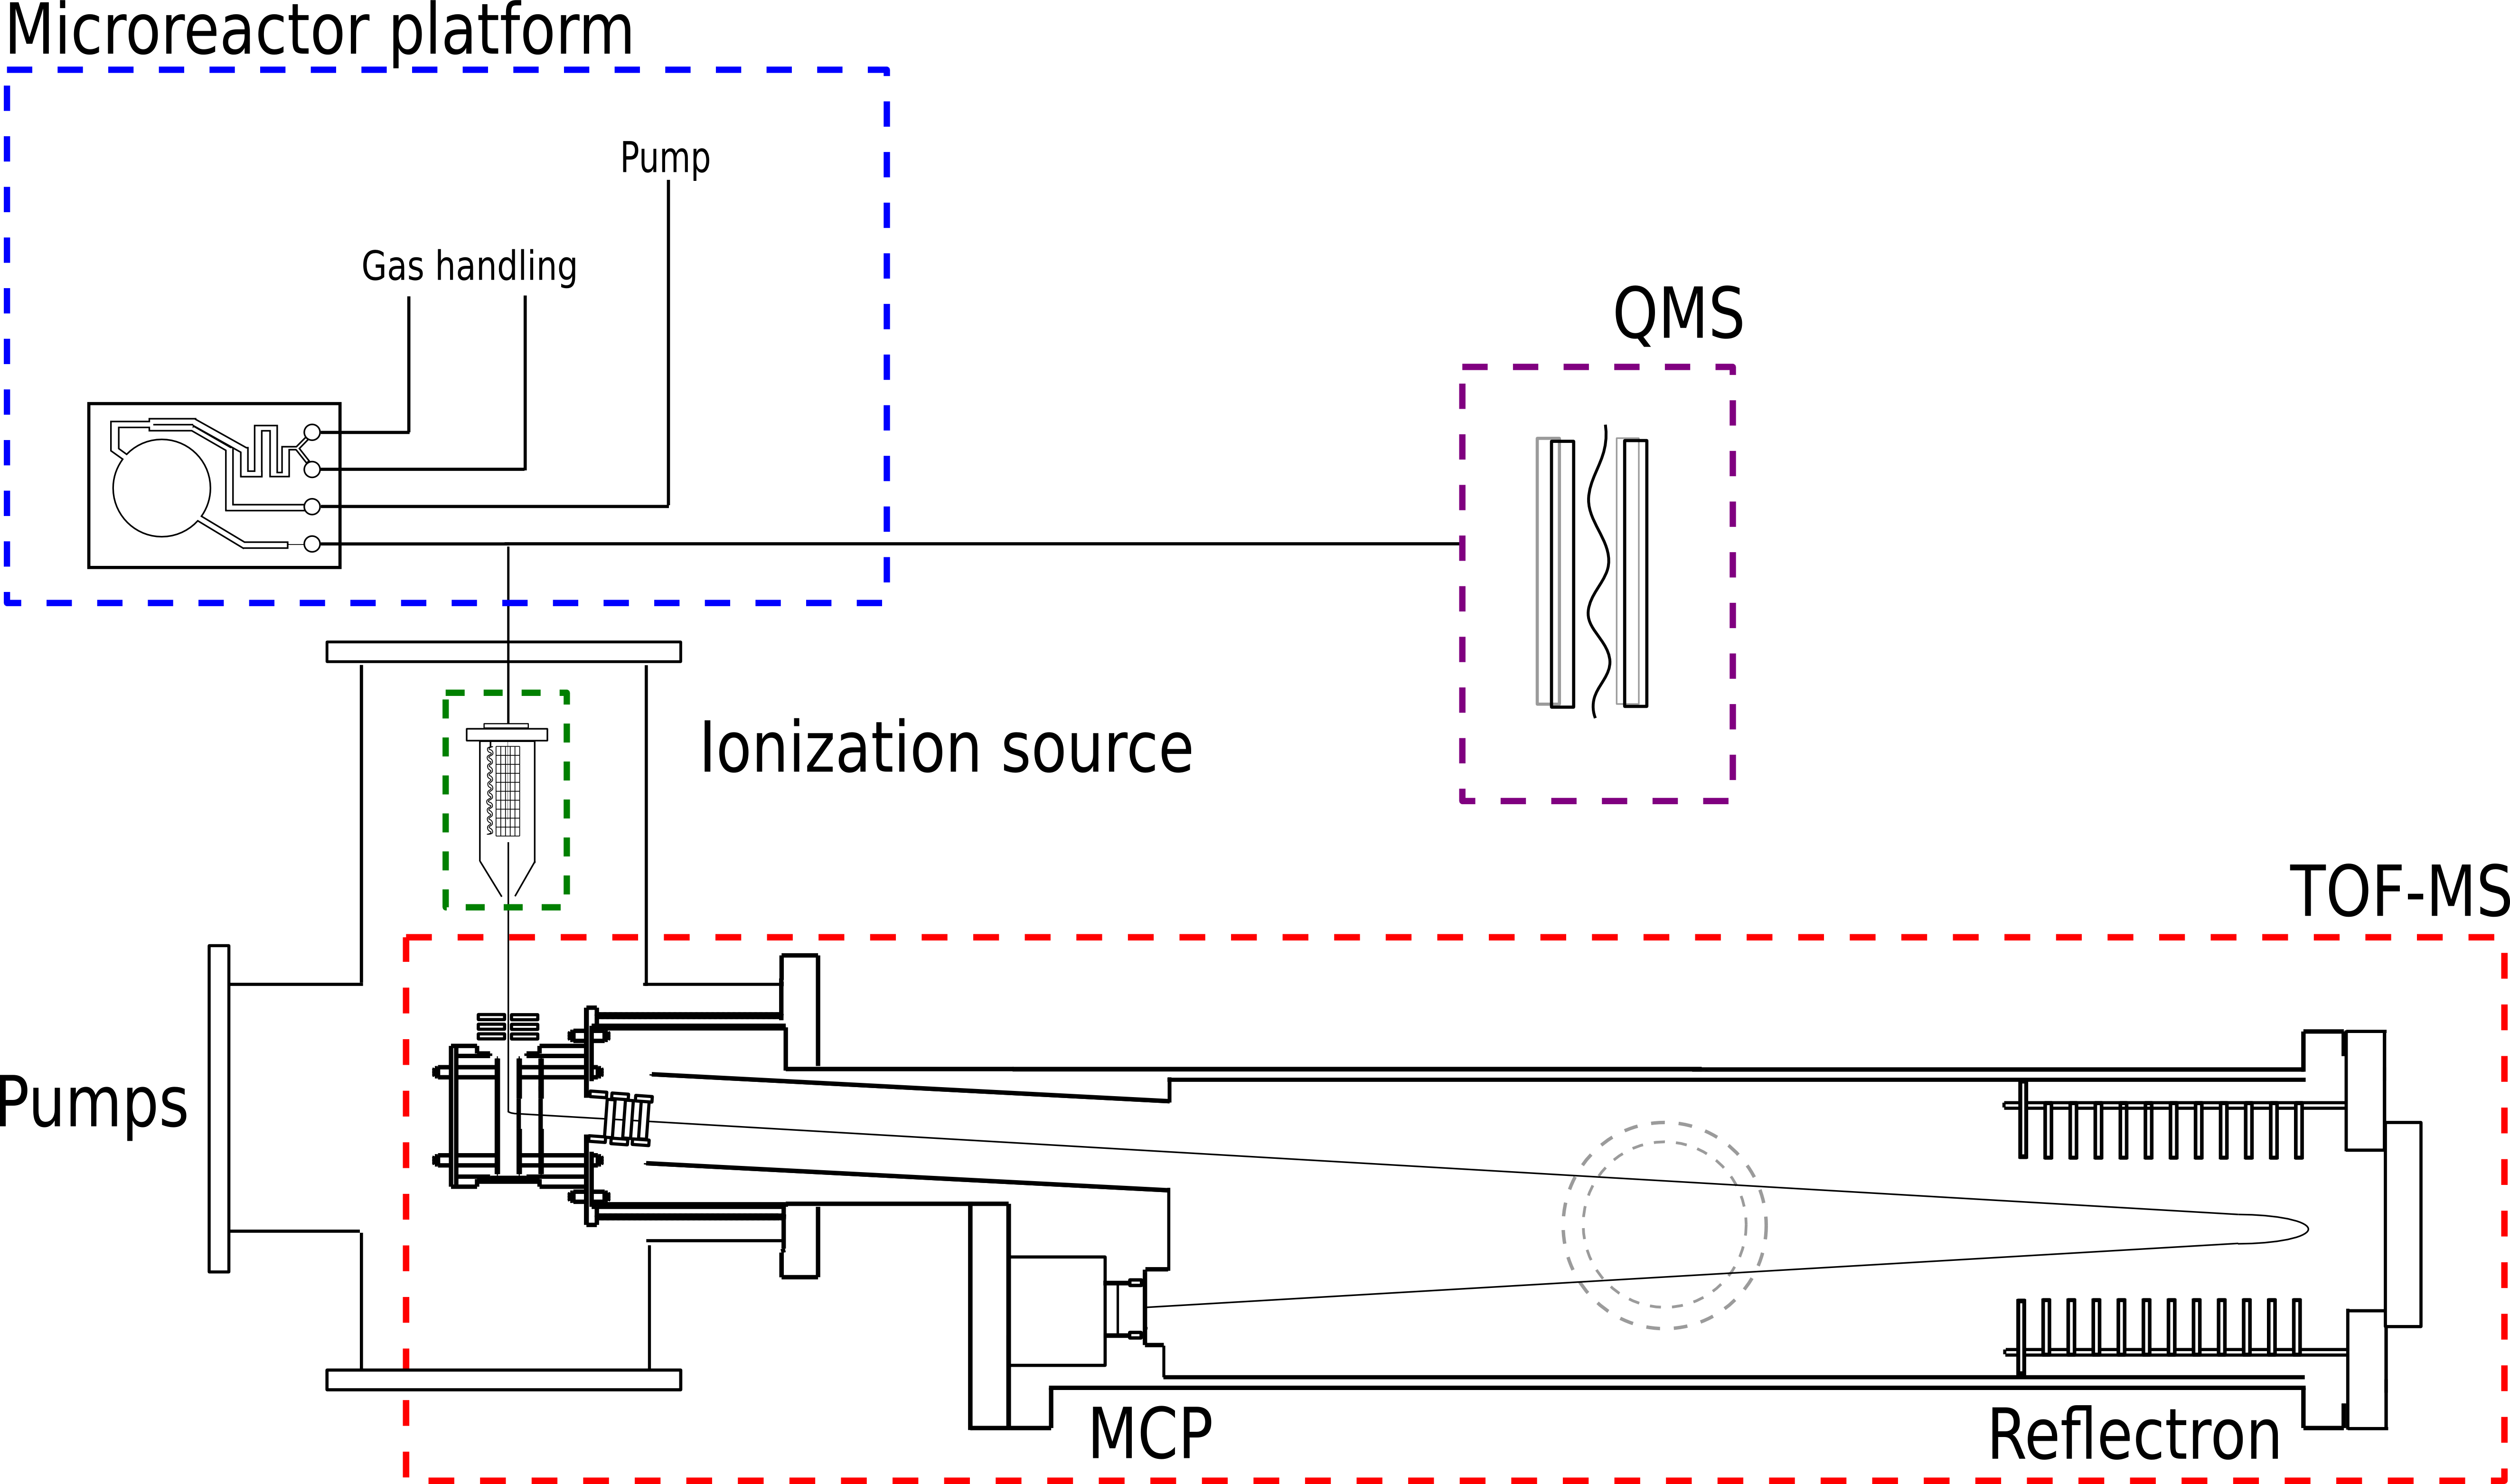
\includegraphics[width=14cm]{TOF_microreactor.png}%
 \caption{Schematic of the total system (not to scale)\label{fig:TOF_microreactor}}%
\end{figure}
The setup consists of three main components. The microreactor, where the catalyst under investigation is deposited, an ionization source which ionizes the gas from the microreactor and the TOF-MS used for gas analysis. 

\subsection{Microreactor and gas handling}

\subsubsection{The microreactor platform}
Catalyst characterization and performance evaluation was performed in a microreactor platform \cite{Henriksen2009}. The microreactors are fabricated in silicon and measures 20x15\,mm. The reactor consists of two gas inlets, a gas outlet, a reactor volume and a capillary used for probing the gas from the reactor volume. The reactor volume is 3\,$\mu$m deep and 1 cm in diameter corresponding to a 240\,nL volume. The two gas inlets are combined on the chip where the inlet gases mix by diffusion. The capillary is designed such that approximately $3\cdot10^{14}$\,molecules$\cdot$s$^{-1}$ is probed from the reactor volume when operated at 1\,bar. Any surplus of gas from the two inlets that does not enter the reactor volume is directed through the outlet to a turbo pump. The design ensures that all molecules or atoms entering the reactor volume, hence exposed to the catalyst under investigation, is detected by mass spectrometry ensuring high sensitivity.

The microreactor is heated by joule heating of a 50 nm platinum strip evaporated through a shadow mask on the backside of the chip. The heating element is contacted by two pogo pins which is connected to a power supply. Additionally, two extra contacts are placed on the chip which facilitates 4 wire measurement of the resistance of the heating element. The heating strip is hence used as a resistance temperature detector (RTD) to monitor the temperature of the chip. At the current configuration temperatures from room temperature to approximately 450\,$^{\circ}$C can be reached.


\subsubsection{Gas handling}
The two gas inlets on the microreactor chip is connected to a gas handling system. A total of 6 gases with accompanying flow controllers are used to control the inlet gas flow to the microreactor. Currently, the system is configured in a 4+2 setup where 4 gases are connected to the one inlet and to gases on the other inlet. All valves and flow controllers are interfaced to computer enabling remote control of the system and the possibility to run experiments over several days without human intervention.

\subsection{Time of flight}
The time of flight equipment used for detection of gas molecules flowed through the capillary of the microreactor is designed as an orthogonal mass spectrometer. The TOF-MS is assembled from modules purchased from Jordan TOF Products, Inc. 

Ionized ions enter the source through a series of entry Einzel lenses used for focusing the beam hence minimizing divergence. In the source the beam is pushed into the flight tube by an the initial repelling push voltage, V$_p$. The ions are further accelerated from ground potential to the liner potential, V$_L$, which is the drift voltage of the flight tube. At the end of the flight tube a reflectron is installed which has two primary purposes. The effective drift length is increased hence increasing resolution of the TOF-MS. The reflectron also works as a focusing lens compensating for any initial velocity dispersion of the ions, i.e. ions with an initial higher velocity will have an increased flight length compared to slower ions. The microchannel plate (MCP) used for ion detection is placed in the focal point of the reflectron giving maximum compensation for initial velocity dispersion. The theoretical resolution of the equipment is $\Delta$m/m$\sim$4000.


In Figure \ref{fig:untreated_data} an example spectrum of a methanol and atmospheric air mixture is shown. Here the high resolution of the TOF-MS is demonstrated by resolution of methanol (CH$_3$OH) and molecular oxygen (O$_2$) which have a mass difference of 43\,milliamu.
\begin{figure}
 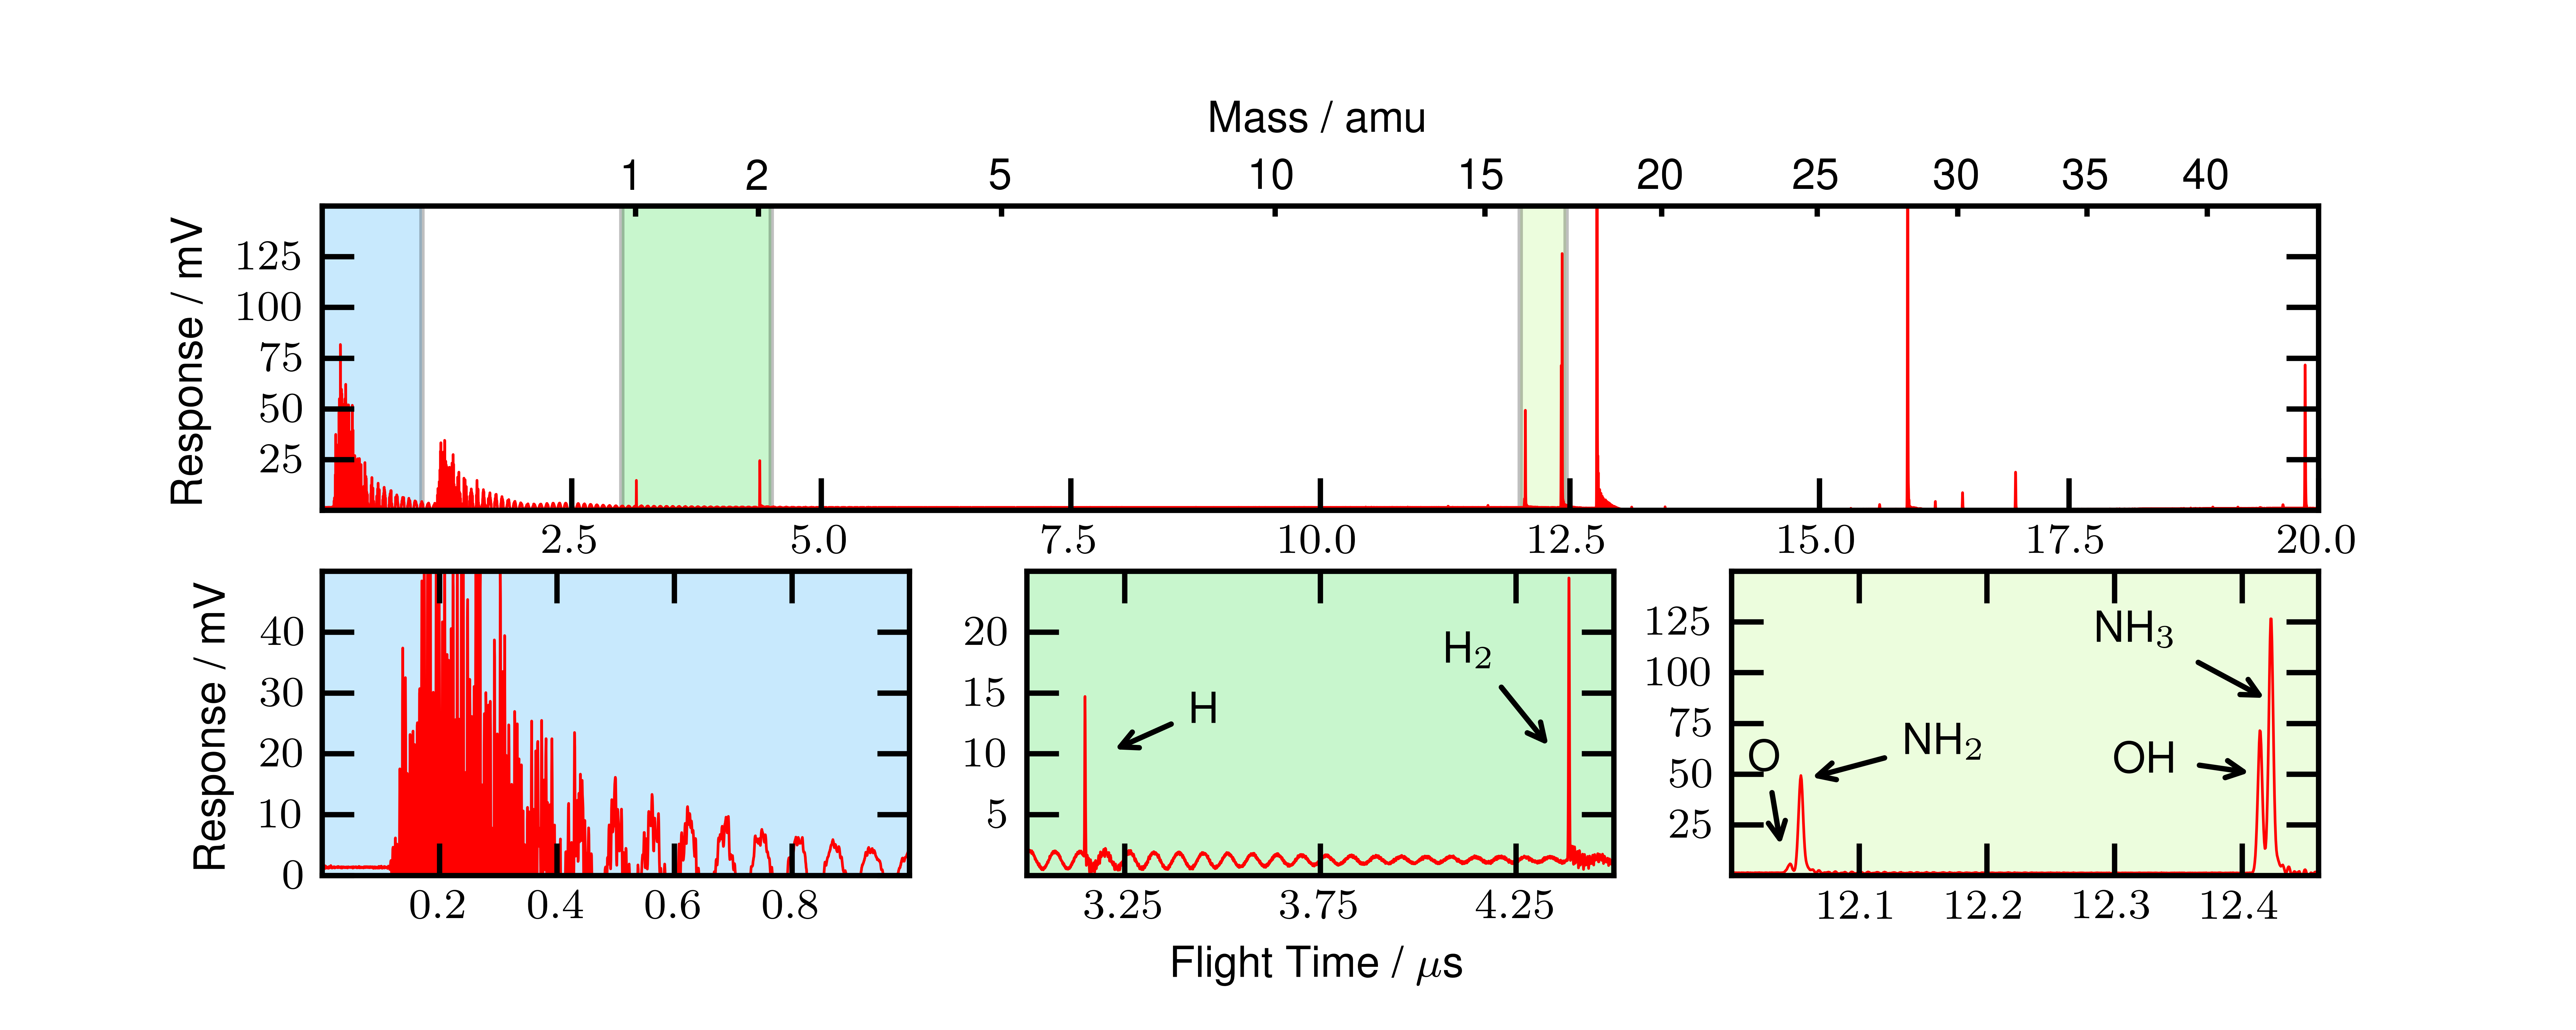
\includegraphics[width=16cm]{untreated_data.png}%
 \caption{Raw data acquired from the TOF-MS in a gas mixture of methanol and atmospheric air. Subfigures show the three different regions of the spectrum. From the first subfigure a delay of the approximately 150\,ns can be seen which is due to delays in cables and the rise time of the repeller pulser. From the center subfigure it is evident that 1\,amu corresponds to approximately 350\,ns difference in flight time in our system. From the last subfigure a zoom of the methanol and molecular oxygen (43\,milliamu mass difference) region is shown.\label{fig:untreated_data}}%
\end{figure}


\subsubsection{Ionization of gas}
As ionization source of the gas flow from the microreactor capillary a modified nude UHV Bayard-Alpert ion gauge is used. Approximately 3\,A is run through the filament resulting in 10\,mA emission current. The grid is biased approximately 40\,V negative compared to the filament to accelerate electrons emitted from the filament towards the grid. Contrary to standard operation of a ion gauge the collector in the center of the grid is short-circuited to the grid ensuring homogeneous field distribution within the grid. To allow ionized ions to escape from the gauge the lid of the grid has been removed \cite{Nottingham1955}. Using this configuration approximately half of the ionized ions are expected to leave the ionization gauge. The entire construction is placed in a nozzle which is differentially pumped by a turbo pump. Large amounts of gas can hence be dosed locally around the ion gauge while still maintaining a low pressure in the source region of the TOF-MS. The nozzle is essential in the setup to avoid high pressure in the source region resulting in a increase in dead counts on the MCP thus decreasing the noise to signal ratio of the recorded signal.

\subsubsection{Data treatment}
A raw data plotted with accompanying gaussian fits are shown in Figure \ref{fig:gaussian_fit}.
\begin{figure}
 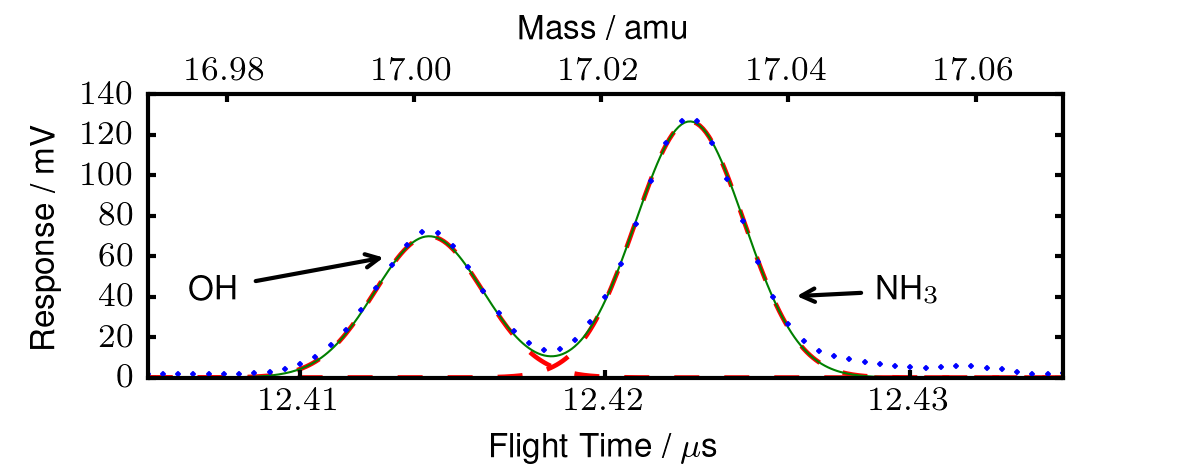
\includegraphics[width=14cm]{ammonia_OH_gauss_fit.png}%
 \caption{Example of two gaussian fits to a double peak consisting of NH$_{3}^{+}$ and OH$^{-}$ both at approximately 17\,amu demonstrating the resolution of the TOF-MS. The entire graph section represents a mass difference of 100\,m-amu.\label{fig:gaussian_fit}}%
\end{figure}
The TOF-MS has furthermore the advantage of a high dynamic range compared to eg. a QMS. In Figure \ref{fig:dynamic_range} raw data from water, hydrogen and oxygen is shown. Without changing any the MCP voltage all the peaks are clearly visible although the ratio of the oxygen to water amplitude is roughly a factor of 4000. 
\begin{figure}
 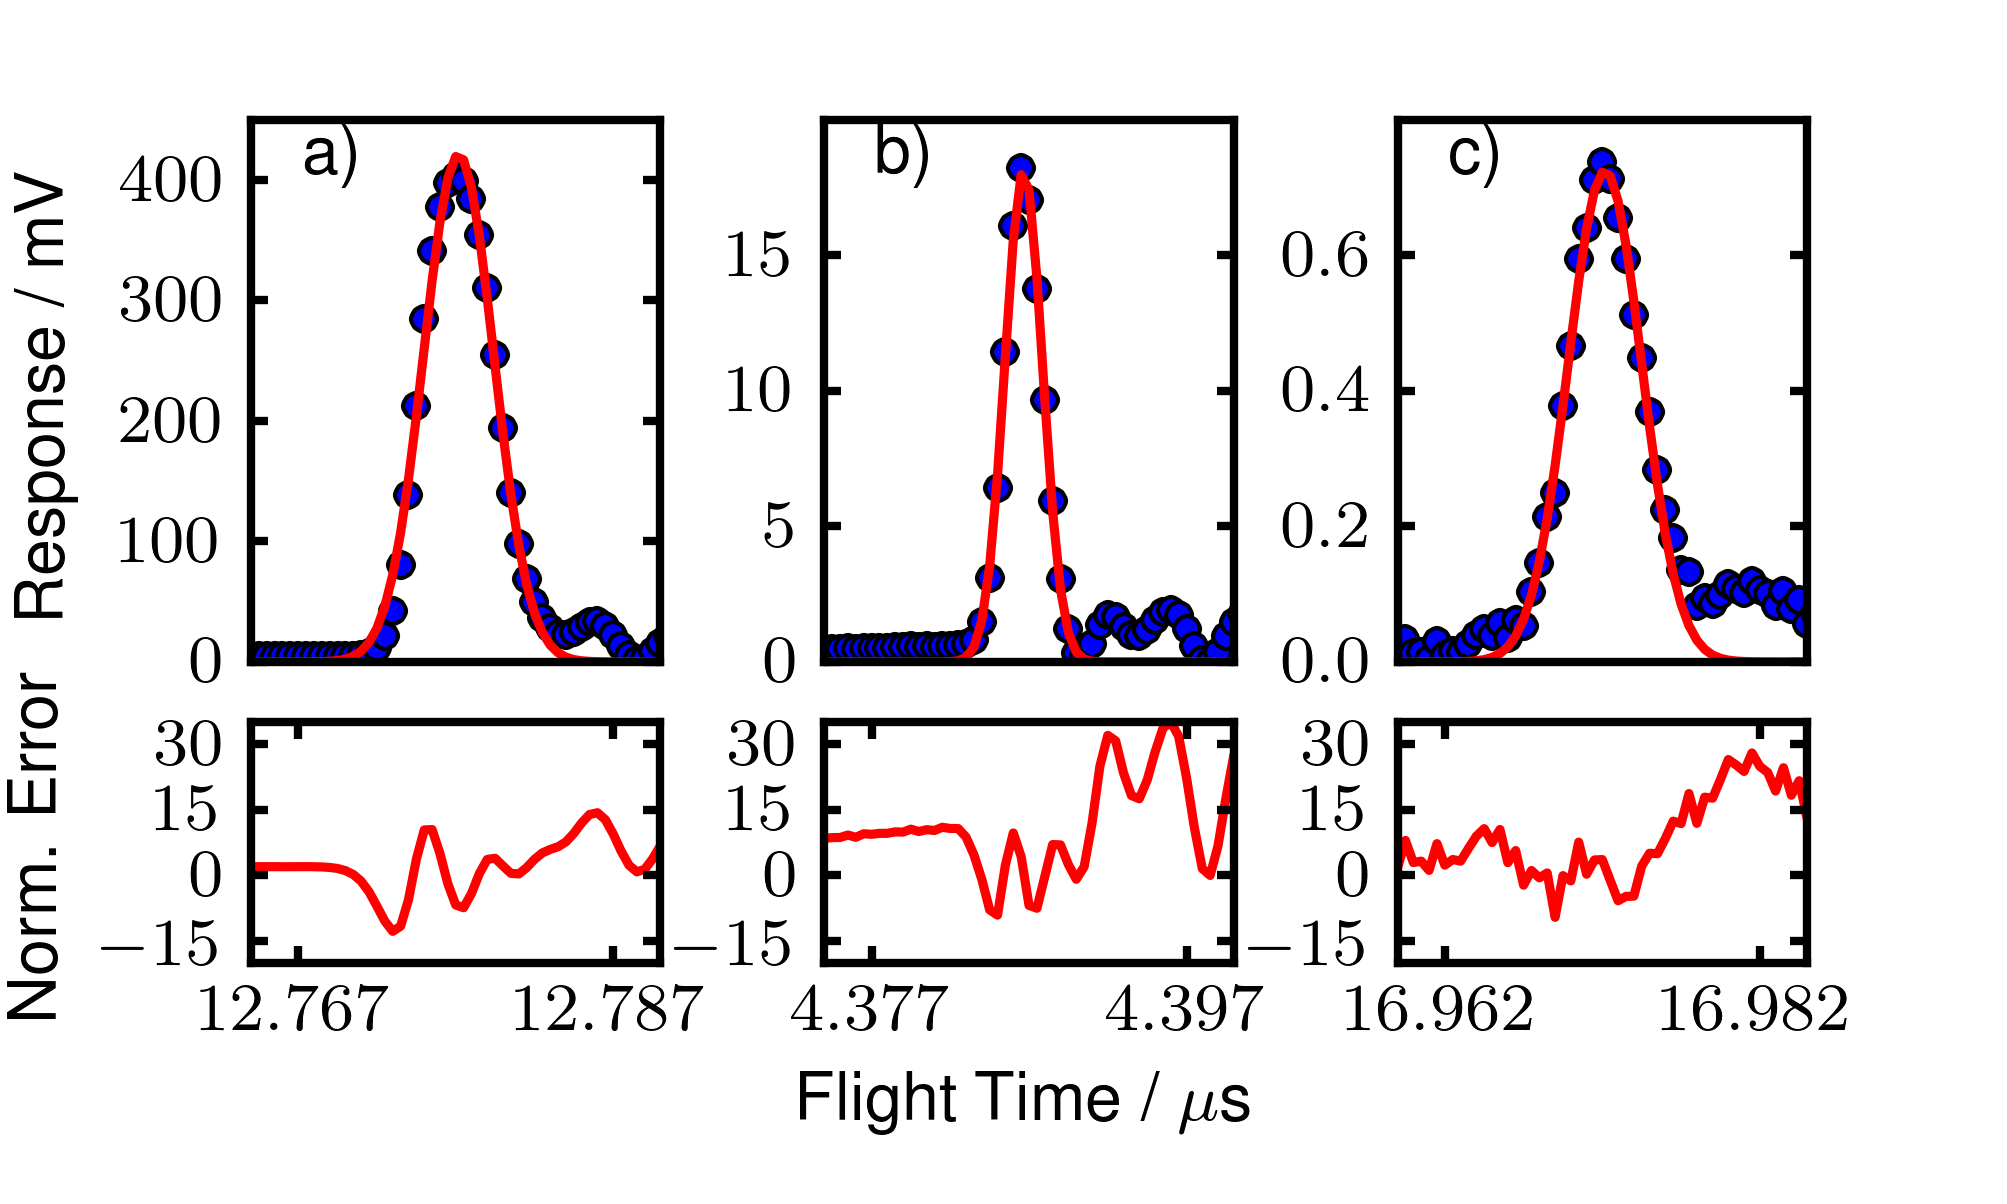
\includegraphics[width=14cm]{dynamic_range.png}%
 \caption{Gaussian fits to three different mass to charge ratios from the same mass spectrum. As seen from the response a high dynamic range of the TOF-MS all yielding good gaussian fits. The TOF-MS can hence be used to monitor both very small and very large signal masses with high time resolution.\label{fig:dynamic_range}}%
\end{figure}

\section{Oxidation of ammonia}
To demonstrate the system capability ammonia oxidation on platinum thin films has been used as test reaction. The catalytic oxidation of ammonia can proceed along primarily three different routes.
\begin{equation}
4NH_3+3O_2\rightarrow 2N_2 + 6H_2O
\label{eq:Pt_clean_combustion}
\end{equation}
\begin{equation}
2NH_3+2O_2\rightarrow N_2O + 3H_2O
\end{equation}
\begin{equation}
4NH_3+5O_2\rightarrow 4NO + 6H_2O
\end{equation}
All of these systems are difficult to analyze both qualitatively and quantitatively by a QMS due to the overlap of NH$_3$, which is a reactant, and OH$^-$ which is a cracking product from H$_2$O, which is a product from the combustion. Specifically, hydroxyls (OH$^{+}$) from cracking of trace water in the system and the combustion reaction and the primary peak of ammonia (NH$_{3}^{+}$) is both detected at m/q$\simeq$17 in a QMS. The low mass resolution of a QMS is typically not adequate to separate the two contributions resulting i difficult analysis. Often a charge to mass ratio without cracking from either products or residue gas in the system is used to be able to detect the amount of ammonia and water. In the case of ammonia, m/q=15 or m/q=8.5 is typically chosen. The monitoring of other than the primary mass to charge ratio due to mass overlap is generally not wanted due to a lower signal to noise ratio of cracking masses. This in turns affect the detection limit of the given mass. Due the acquisition of entire mass spectra with high time resolution instead of monitoring individual masses by QMS the TOF-MS is not limited to unique signature masses resulting in higher signal to noise ratio spectra.
\begin{figure}
 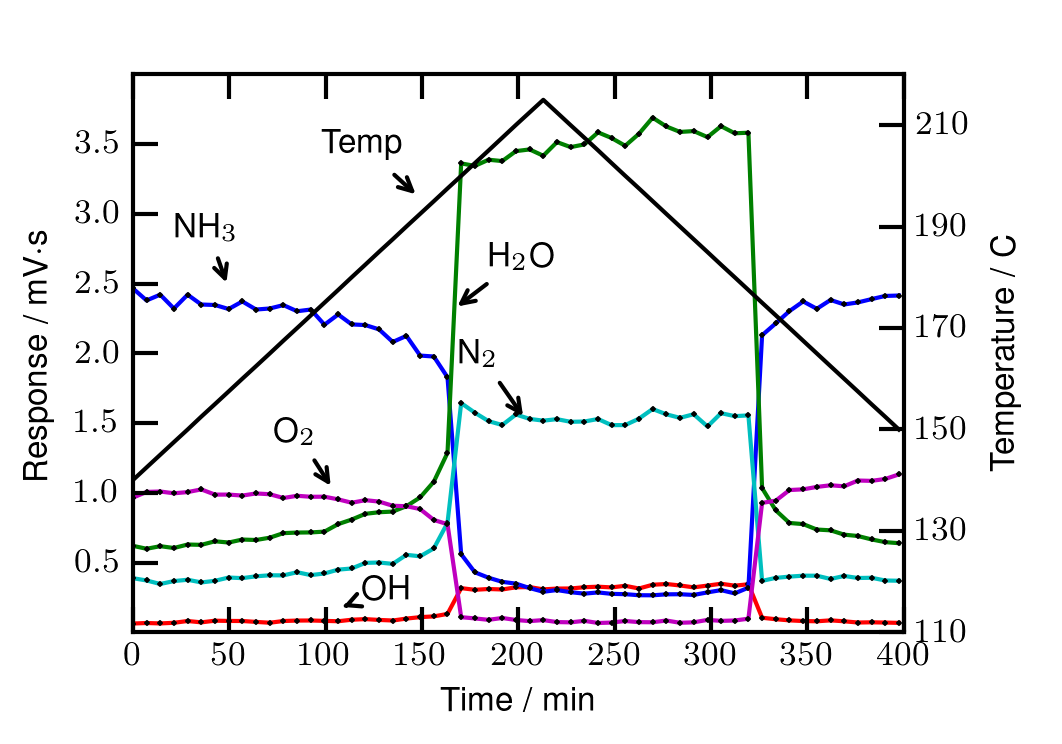
\includegraphics[width=14cm]{ammonia_reactivity.png}%
 \caption{Ammonia oxidation as a function of temperature on a Pt thin film. As the temperature is increased ammonia is oxidized to H$_2$O and N$_2$. Furthermore, the OH and NH$_3$ signal is anticorrelated demonstrating the ability to resolve these masses.\label{fig:ammonia_reactivity}}%
\end{figure}
In Figure \ref{fig:ammonia_reactivity} a number of masses as a function of time are shown. At experiment start the microreactor is equilibrated with a stoichiometric mix of NH$_3$ and O$_2$ (3:4). Hereafter the temperature is increased while TOF spectra are acquired. Spectra were acquired from triggering of the acceleration pulse up to 25\,$\mu$s of flight time corresponding to a maximum of 70 amu in our system. 

For ammonia oxidation both N$_2$O (m/q = 44), NO (m/q = 30) and NO$_2$ (m/q = 46) are of interest. 



\section{Summary}

\section{Acknowledgements}

% If in two-column mode, this environment will change to single-column format so that long equations can be displayed. 
% Use only when necessary.
%\begin{widetext}
%$$\mbox{put long equation here}$$
%\end{widetext}

% Figures should be put into the text as floats. 
% Use the graphics or graphicx packages (distributed with LaTeX2e).
% See the LaTeX Graphics Companion by Michel Goosens, Sebastian Rahtz, and Frank Mittelbach for examples. 
%
% Here is an example of the general form of a figure:
% Fill in the caption in the braces of the \caption{} command. 
% Put the label that you will use with \ref{} command in the braces of the \label{} command.
%
% \begin{figure}
% \includegraphics{}%
% \caption{\label{}}%
% \end{figure}

% Tables may be be put in the text as floats.
% Here is an example of the general form of a table:
% Fill in the caption in the braces of the \caption{} command. Put the label
% that you will use with \ref{} command in the braces of the \label{} command.
% Insert the column specifiers (l, r, c, d, etc.) in the empty braces of the
% \begin{tabular}{} command.
%
% \begin{table}
% \caption{\label{} }
% \begin{tabular}{}
% \end{tabular}
% \end{table}

% If you have acknowledgments, this puts in the proper section head.
%\begin{acknowledgments}
% Put your acknowledgments here.
%\end{acknowledgments}

% Create the reference section using BibTeX:
\bibliographystyle{abbrv}
%\bibliographystyle{alpha}
%\bibliographystyle{plain}
\bibliography{literature}

\end{document}
%
% ****** End of file aiptemplate.tex ******
